\documentclass{article}

\textwidth=6.5in
\textheight=8.5in
\voffset=-54pt
\oddsidemargin=0in
\evensidemargin=0in
\setlength{\parskip}{8pt}
\setlength{\parindent}{0pt}

\usepackage{workbook}

\usepackage[]{handout}

\begin{document}

\begin{center}
  \large\textsc{Problem Set 13 - Inverse Trig Functions}
  
      \pspace{12pt}
  \begin{problemonly}\large Name: \rule{5cm}{0.15mm}\\ \end{problemonly}
\end{center}

\begin{framed}
\textbf{Definitions:}
      \begin{itemize}[topsep=0pt]
        \item $\arccos x$ is the angle in the interval $\fitb{1in}{[0,\pi]}$ 
        whose cosine is $x$.

        The domain of $\arccos$ is $\fitb{1in}{[-1,1]}$ 
        and the range is $\fitb{1in}{[0,\pi]}$.
        
        \item $\arcsin x$ is the angle in the interval $\fitb{1in}{[\frac{-\pi}{2},
        \frac{\pi}{2}]}$ whose sine is $x$.

        The domain of $\arcsin$ is $\fitb{1in}{[-1,1]}$ 
        and the range is $\fitb{1in}{[\frac{-\pi}{2},
        \frac{\pi}{2}]}$.
        
        \item $\arctan x$ is the angle in the interval $\fitb{1in}{(\frac{-\pi}{2},
        \frac{\pi}{2})}$ whose tangent is $x$.

        The domain of $\arctan$ is $\fitb{1in}{(-\infty,\infty]}$ 
        and the range is $\fitb{1in}{(\frac{-\pi}{2},
        \frac{\pi}{2})}$.
      \end{itemize}
\end{framed}
\vspace{-8pt}
\begin{warmup}
  This first problem, {\#W1}, is a warm-up.  The
  answers are upside-down at the bottom of 
  the page so that you can make sure
  you're comfortable with how the inverse trigonometric functions are
  defined before you do the rest of the problem set. Your work on this problem will
  not be graded. 

  \begin{enumerate}[topsep=0pt,label=W\arabic*., ref=\#W\arabic*]
  \item 

 Evaluate the following, or say that they are undefined. 

 \probonly{
 \begin{tasks}[after-item-skip=90pt, label=(\alph*)](3)
 \task $\arcsin (-1)$
 \task $\arccos (-1)$
 \task $\tan^{-1}(-1)$

 \task $\arcsin(\frac{\sqrt{2}}{2})$
 \task $\cos^{-1}(\sqrt{3})$
 \task $\arctan(\sqrt{3})$

 \task $\sin^{-1}(-\frac{\sqrt{2}}{2})$
 \task $\arccos(-\frac{1}{2})$
 \task $\arctan(-\frac{\sqrt3}{3})$
 
 \end{tasks}
 }

 \solonly{

      \begin{enumerate}
      \item
\begin{problem}
          $\arcsin (-1) \vphantom{\left( \frac{1}{\sqrt{1}}
            \right)}$
        \end{problem}
        \pspace{0.4in}

        \begin{solution}
          This is defined to be the angle in $\left[ - \frac{\pi}{2},
            \frac{\pi}{2} \right]$ whose sine is $-1$; the single such angle
          is $\boxed{- \dfrac{\pi}{2}}$.  (So, for example, even though
          $\sin \frac{3 \pi}{2} = -1$, $\arcsin(-1) \neq - \frac{3
            \pi}{2}$.)
        \end{solution}

      \item
\begin{problem}
          $\arccos (-1) \vphantom{\left( \frac{1}{\sqrt{1}}
            \right)}$
        \end{problem}
        \pspace{0.4in}

        \begin{solution}
          This is the angle in $[0, \pi]$ whose cosine is $-1$; that angle is
          \fbox{$\pi$}. 
        \end{solution}

      \item
\begin{problem}
          $\tan^{-1} (-1) \vphantom{\left( \frac{1}{\sqrt{1}}
            \right)}$
        \end{problem}

        \begin{solution}
          This is the angle in $\left( - \frac{\pi}{2}, \frac{\pi}{2}
          \right)$ whose tan is $-1$; that angle is 
          $\boxed{-\dfrac{\pi}{4}}$. 
        \end{solution}

      \item
        \begin{problem}
          $\cos^{-1} (\sqrt{3}) \vphantom{\left(
              \frac{1}{\sqrt{1}} \right)}$
        \end{problem}
        \pspace{0.4in}

        \begin{solution}
          This is the angle in $[0, \pi]$ whose cosine is $\sqrt{3}$, but
          there is no such angle: cosine of any angle must be between $-1$
          and $1$.  So, this is \fbox{undefined}.
        \end{solution}
        

      \item
        \begin{problem}
          $\arctan (\sqrt{3}) \vphantom{\left(
              \frac{1}{\sqrt{1}} \right)}$
        \end{problem}
        \pspace{0.4in}

        \begin{solution}
          This is the angle in $\left( - \frac{\pi}{2}, \frac{\pi}{2}
          \right)$ whose tangent is $\sqrt{3}$; that angle is
          $\boxed{\frac{\pi}{3}}$. 
        \end{solution}

      \item
        \begin{problem}
          $\sin^{-1}(\frac{\sqrt2}{2})$
        \end{problem}

        \begin{solution}
          This is the angle in $\left[ - \frac{\pi}{2}, \frac{\pi}{2}
          \right]$ whose sine is $\frac{\sqrt{2}}{2}$; that angle is
          $\boxed{\frac{\pi}{4}}$. 
        \end{solution}

    \item
    \begin{problem}
        $\arcsin(-\frac{1}{\sqrt2})$
    \end{problem}
    \pspace{0.4in}

    \begin{solution}
        This is the angle in $[-\pi/2,\pi/2]$ whose sine is $-1/\sqrt2$;
        that angle is $\boxed{-\frac{\pi}{4}}$.
    \end{solution}

    \item
    \begin{problem}
        $\arccos(-\frac{1}{2})$
    \end{problem}
    \pspace{0.4in}

    \begin{solution}
        This is the angle in $[0,\pi]$ whose cosine is $-1/2$.
        This angle is $\boxed{\frac{2\pi}{3}}$.
    \end{solution}

    \item
    \begin{problem}
        $\arctan(-\frac{\sqrt3}{3})$
    \end{problem}

    \begin{solution}
        This is the angle in $[-\pi/2,\pi/2]$ whose tangent is $-\sqrt3/3$.
        This angle is  $\boxed{-\frac{\pi}{6}}$.
    \end{solution}

      \end{enumerate}    
}

  \end{enumerate}
  \pspace{0.6in}

\probonly{
\vfill
  \rotatebox{180}{
  \textbf{W1.} 
  \textbf{(a)} $-\pi/2$
  \textbf{(b)} $\pi$
  \textbf{(c)} $-\pi/4$
  \textbf{(d)} $\pi/4$
  \textbf{(e)} undefined
  \textbf{(f)} $\pi/3$
  \textbf{(g)} $-\pi/4$
  \textbf{(h)} $2\pi/3$ 
  \textbf{(i)} $-\pi/6$}
  }
  \vspace{4pt}
\end{warmup}
\probonly{
The graded problems begin on the next page.}
\pspace{\newpage}
\begin{enumerate}[topsep=0pt]
\item 

\begin{grading}
 15 points:   3/3/2/7.
\end{grading}

You may wish to review pp. 645-647 in Gottlieb if you get stuck at any point on this problem set.

  \begin{enumerate}[topsep=0pt]
  \item
\begin{problem}[\stretch{3}]
      Sketch the graph of $\cos x$ on $[0, \pi]$.  Label at least 3 points
      on the graph with exact coordinates, and make sure the range of your
      graph is clear.
    \end{problem}

    \begin{solution} 
      Here's the graph; its range is $[-1, 1]$:
      \begin{center}
        \begin{tikzpicture}
          \begin{axis}[xtick={-4.71239, -3.14159, -1.5708, 0., 3.14159,
              4.71239}, xticklabels={$-\frac{3 \pi }{2}$, $-\pi$,
              $-\frac{\pi }{2}$, $0.$, $\pi$, $\frac{3 \pi }{2}$},
            ytick={-4.71239, -3.14159, -1, 0., 3.14159, 4.71239},
            yticklabels={$-\frac{3 \pi }{2}$, $-\pi$, $-1$, $0.$, $\pi$,
              $\frac{3 \pi }{2}$}, xmin=-3.5, xmax=3.5, ymin=-3.5,
            ymax=3.5, clip=false]            
            \addplot[domain=0:3.15] {cos(deg(x))};
            \addplot[only marks, mark=*, mark size=1.5pt] coordinates
            {
              (0, 1)
              (1.0472, 0.5)
              (1.5708, 0)
              (3.14159, -1)
            }
            node[pos=0, left] {$(0, 1)$}
            node[pos=0.333, anchor=south west, inner sep=1pt] {$\left( \frac{\pi}{3}, \frac{1}{2} \right)$}
            node[pos=0.667, anchor=north east, inner sep=1pt] {$\left( \frac{\pi}{2}, 0
              \right)$}
            node[pos=1, right] {$(\pi, -1)$}
            ;
          \end{axis}
        \end{tikzpicture}
      \end{center}      
    \end{solution}

  \item
    \begin{problem}
      As we know, $\arccos x$, also written $\cos^{-1} x$, is defined to
      be the angle in $[0, \pi]$ whose cosine is $x$.  Use your sketch in
      {{{{\#1}}(a)}} to sketch the graph of $\arccos x$ on the same axes.  Label the coordinates of at least 3
      points on the graph, and make sure the domain and range of your
      graph are clear.
    \end{problem}

    \begin{solution}
      This is simply the inverse of the graph we drew in
      {{{{\#1}}(a)}}:
      \begin{center}
        \begin{tikzpicture}
          \begin{axis}[xtick={-4.71239, -3.14159, -1.5708, 0., 1.5708,
              3.14159, 4.71239}, xticklabels={$-\frac{3 \pi }{2}$, $-\pi$,
              $-\frac{\pi }{2}$, $0.$, $\frac{\pi }{2}$, $\pi$, $\frac{3
                \pi }{2}$}, ytick={-4.71239, -3.14159, -1.5708, 0.,
              1.5708, 3.14159, 4.71239}, yticklabels={$-\frac{3 \pi }{2}$,
              $-\pi$, $-\frac{\pi }{2}$, $0.$, $\frac{\pi }{2}$, $\pi$,
              $\frac{3 \pi }{2}$}, xmin=-3.5, xmax=3.5, ymin=-3.5,
            ymax=3.5, clip=false]
            \addplot[domain=0:3.14159, red] {cos(deg(x))}
            node[right]{$\cos x$};
            \addplot[domain=-1:1, blue] {rad(acos(x))}
            node[pos=0.2, left]{$\arccos x$};
            \addplot[only marks, mark=*, blue, mark size=1.5pt] coordinates
            {
              (1, 0)
              (0.5, 1.0472)
              (0, 1.5708)
              (-1, 3.14159)
            }
            node[pos=0, below]{$(1, 0)$}
            node[pos=0.333, right] {$\left( \frac{1}{2}, \frac{\pi}{3} \right)$}
            node[pos=0.667, anchor=south west, inner sep=1pt] {$\left(0, \frac{\pi}{2} \right)$}
            node[pos=1, above]{$(-1, \pi$)};            
          \end{axis}
        \end{tikzpicture}
      \end{center}
    \end{solution}

  \item
    \begin{problem}[\stretch{1}]
      What are the domain and range of $\arccos x$?  (Now that you've
      graphed $\arccos x$, this should be straightforward to answer from
      your graph.)
    \end{problem}

    \begin{solution}
      The domain of $\arccos x$ is $[-1, 1]$, and the range is $[0,
      \pi]$. 
    \end{solution}

  \item
    \begin{problem}
      Fill in the following table of values for $\arccos$.  (One value
      is undefined.)
    \end{problem}

    \begin{problemonly}
      \begin{center}
        \renewcommand{\arraystretch}{2.5}
        \newcolumntype{M}[1]{>{\centering\arraybackslash}m{#1}}
        \newcolumntype{N}{@{}m{0pt}@{}}
        \begin{tabular}{|M{0.5in}||M{0.5in}|M{0.5in}| M{0.5in}|M{0.5in}|M{0.5in}|M{0.5in}|
        M{0.5in}|N}
          \hline
          $\bm{x}$  & $-1$ &
          $-\dfrac{\sqrt{3}}{2}$ &
          $-\dfrac{1}{2}$ & $0$ &
          $\dfrac{\sqrt{2}}{2}$ &
          $1$ & $3$ &\\[4pt]
          \hline
          $\bm{\arccos x}$ &  & & & & & & &\\[16pt]
          \hline      
        \end{tabular}
      \end{center}
    \end{problemonly}

    \renewcommand{\arraystretch}{1}

    \probonly{\emph{Do these agree with your work in the previous parts of
        this problem?}}

    \begin{solution}
      \begin{center}
        \renewcommand{\arraystretch}{2.5}
        \begin{tabular}{|l|*{9}{|>{$}m{0.4in}<{$}}|}
          \hline
          $\bm{x}$ & -1 & - \dfrac{\sqrt{3}}{2} & -
          \dfrac{1}{2} & 0 & \dfrac{\sqrt{2}}{2} & 1 & 3 \\
          \hline
          $\bm{\arccos x}$ & \pi & \dfrac{5\pi}{6} &
          \dfrac{2\pi}{3} & 
          \dfrac{\pi}{2} & \dfrac{\pi}{4} & 0 & \text{undef.}\\
          \hline      
        \end{tabular}
      \end{center}
      % \renewcommand{\arraystretch}{1}
    \end{solution}

  \end{enumerate}

  \pspace{\newpage}

\item 

\begin{grading}
 10 points:   4/1/4/1.
\end{grading}

 %(variant of 20.3.3)% 20.3.3

  \begin{enumerate}

  \item
\begin{problem}[\stretch{3}]
      Graph $y=\arctan x$. What is its domain?  Its range?
    \end{problem}

    \begin{solution}
      Here is the graph of $\arctan x$ (see
        {{\#4}} on the worksheet for more explanation):
      \begin{center}
        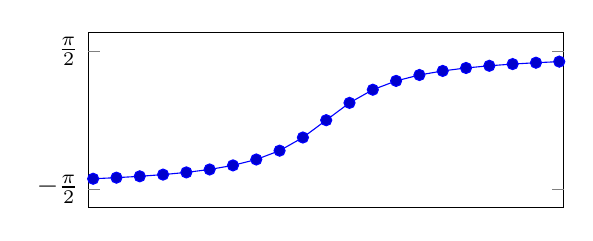
\begin{tikzpicture}
          \begin{axis}[xtick=\empty, ytick=\empty, extra y ticks={-1.5708,
              1.5708}, extra y tick labels={$-\frac{\pi}{2}$,
              $\frac{\pi}{2}$}, xmin=-4.25, xmax=4.25, width=3in,
            height=1.5in, ymin=-2, ymax=2] % 
            \addplot+[blue, solid]{rad(atan(x))};
          \end{axis}
        \end{tikzpicture}
      \end{center}
      The domain is $(-\infty, \infty)$, and the range is
      $\left(-\frac{\pi}{2}, \frac{\pi}{2} \right)$.
    \end{solution}

  \item
    \begin{problem}[\stretch{1}]
      Is $\arctan x$ an even function, an odd function, or neither?
    \end{problem}

    \begin{solution}
      From the graph, we see that $\arctan x$ is an odd function. 
    \end{solution}

  \item
    \begin{problem}[\stretch{3}]
      At this point, we don't know how to take the derivative of $\arctan
      x$ directly. Nonetheless, by looking at the graph of $\arctan
      x$, sketch its derivative.  Where is the derivative positive?
      Negative?
    \end{problem}

    \begin{solution}
      From {{{{\#2}}(a)}}, $\arctan x$ is always increasing, so
      \fbox{its derivative is always positive}.  The graph of $\arctan x$
      flattens out as it approaches its horizontal asymptotes, so the
      derivative is close to 0 when $x$ is very positive or very negative.
      The graph of $\arctan x$ appears steepest at $x = 0$, so the
      derivative will be highest there.  Putting this all together, here's
      the graph of the derivative of $\arctan x$:
      \begin{center}
        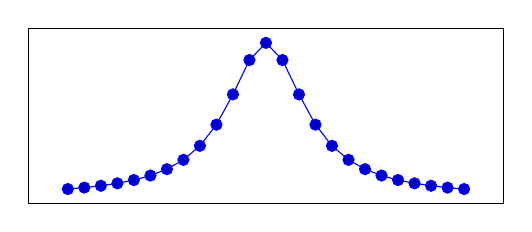
\begin{tikzpicture}
          \begin{axis}[xtick=\empty, ytick=\empty, width=3in, height=1.5in]
            \addplot+[domain=-4.25:4.25] {1 / (1 + x^2)};
          \end{axis}
        \end{tikzpicture}
      \end{center}
    \end{solution}

  \item
    \begin{problem}[\nstretch{1}]
      Is the derivative of $\arctan x$ an even function, an odd function,
      or neither?
    \end{problem}

    \begin{solution}
      The derivative is an \fbox{even function}.
    \end{solution}

  \end{enumerate}

\item 

\begin{grading}
 14 points:   3/3/4/4
\end{grading}

\begin{enumerate}
%   \item Find the following exactly.

%     \probonly{}
%       \begin{enumerate}
%       \item
% \begin{problem}
%           $\displaystyle \arctan\left(\frac{1}{\sqrt{3}}\right)$
%         \end{problem}

%         \begin{solution}
%           This is the angle in $\left( - \frac{\pi}{2}, \frac{\pi}{2}
%           \right)$ whose tan is $\frac{1}{\sqrt{3}}$; that angle is
%           $\boxed{ \frac{\pi }{6}}$.
%         \end{solution}

%       \item
% \begin{problem}
%           $\displaystyle \cos ^{-1}\left(-\frac{1}{\sqrt{2}}\right)$
%         \end{problem}

%         \begin{solution}
%           This is the angle in $[0, \pi]$ whose cosine is
%           $-\frac{1}{\sqrt{2}}$; that angle is $\boxed{ \frac{3 \pi
%             }{4}}$.
%         \end{solution}

%       \item
% \begin{problem}
%           $\displaystyle \arcsin\left(-\frac{\sqrt{3}}{2} \right)$
%         \end{problem}

%         \begin{solution}
%           This is the angle in $\left[ - \frac{\pi}{2}, \frac{\pi}{2}
%           \right]$ whose sine is $- \frac{\sqrt{3}}{2}$; that angle is
%           $\boxed{ - \frac{\pi}{3}}$. 
%         \end{solution}

%       \end{enumerate}    
%       \probonly{}

  \item Find the closest neighboring special angles (multiples of $\frac{\pi}{6},\ \frac{\pi}{4},\ \frac{\pi}{3}$, etc.) for each of the given angles. Use the unit circle to help. The first has been done for you as an example.
  
  It may be useful to know that $\sqrt{3}\approx 1.732$, $\frac{\sqrt3}{2}\approx 0.866$, $\frac{\sqrt2}{2}\approx 0.707$, and $\frac{\sqrt3}{3} \approx 0.577$.

  \pspace{12pt}
  
\begin{multicols}{2}

      \begin{enumerate}
      \vspace{12pt}
      \item
\begin{problem}[0.5in]
$\cfitb[\dfrac{\pi}{3}\vphantom{\dfrac{\pi}{3}}]{0.5in}{\frac{\pi}{3}} < \arcsin (0.9) < \cfitb[\dfrac{\pi}{2}\vphantom{\dfrac{\pi}{3}}]{0.5in}{\frac{\pi}{2}}$ 
        \end{problem}
        
      \item
\begin{problem}[0.5in]
$\cfitb[\vphantom{\dfrac{\pi}{3}}]{0.5in}{\frac{\pi}{4}} < \arccos (0.6) < \cfitb[\vphantom{\dfrac{\pi}{3}}]{0.5in}{\frac{\pi}{3}}$ 
        \end{problem}

      \item
\begin{problem}[0.5in]
$\cfitb[\vphantom{\dfrac{\pi}{3}}]{0.5in}{\frac{\pi}{4}} < \tan^{-1} (1.6) < \cfitb[\vphantom{\dfrac{\pi}{3}}]{0.5in}{\frac{\pi}{3}}$ 
        \end{problem}


      \item
\begin{problem}[0.5in]
$\cfitb[\vphantom{\dfrac{\pi}{3}}]{0.5in}{-\frac{\pi}{6}} < \sin^{-1} (-0.1) < \cfitb[\vphantom{\dfrac{\pi}{3}}]{0.5in}{0}$ 
        \end{problem}

      \item
\begin{problem}[0.5in]
$\cfitb[\vphantom{\dfrac{\pi}{3}}]{0.5in}{\frac{\pi}{2}} < \cos^{-1} (-0.3) < \cfitb[\vphantom{\dfrac{\pi}{3}}]{0.5in}{\frac{2\pi}{3}}$ 
        \end{problem}

      \item
\begin{problem}[0.5in]
$\cfitb[\vphantom{\dfrac{\pi}{3}}]{0.5in}{-\frac{\pi}{6}} < \arctan (-0.4) < \cfitb[\vphantom{\dfrac{\pi}{3}}]{0.5in}{0}$ 
        \end{problem}

\end{enumerate}
\end{multicols}

\begin{solution}
    \begin{enumerate}[label=\roman*.]
        \item $\arcsin(0.9)$ is the angle in $[-\pi/2, \pi/2]$ whose sine is 0.9. Since 0.9 is between $\frac{\sqrt3}{2}$ and $1$, $\arcsin(0.9)$ must be between $\frac{\pi}{3}$ and $\frac{\pi}{2}$.
        \item $\arccos(0.6)$ is the angle in $[0, \pi]$ whose cosine is 0.6. Since 0.6 is between $\frac{1}{2}$ and $\frac{\sqrt{2}}{2}$, $\arccos(0.6)$ must be between $\frac{\pi}{3}$ and $\frac{\pi}{4}$.
        \item $\tan^{-1}(1.6)$ is the angle in $(-\pi/2, \pi/2)$ whose tangent is 1.6. Since 1.6 is between $1$ and $\sqrt{3}$, $\tan^{-1}(1.6)$ must be between $\frac{\pi}{4}$ and $\frac{\pi}{3}$.
        \item $\sin^{-1}(1.6)$ is the angle in $[-\pi/2, \pi/2]$ whose sine is -0.1. Since -0.1 is between $0$ and $-\frac{1}{2}$, $\sin^{-1}(-0.1)$ must be between $0$ and $-\frac{\pi}{6}$.
        \item $\cos^{-1}(-0.3)$ is the angle in $[0, \pi]$ whose cosine is -0.3. Since -0.3 is between $0$ and $-\frac{1}{2}$, $\cos^{-1}(-0.1)$ must be between $\frac{\pi}{2}$ and $\frac{2\pi}{3}$.
        \item $\arctan(-0.4)$ is the angle in $(-\pi/2, \pi/2)$ whose tangent is -0.4. Since -0.4 is between $0$ and $-\sqrt{3}/3$, $\arctan(-0.4)$ must be between $0$ and $-\frac{\pi}{6}$.
    \end{enumerate}
\end{solution}

%       \item
% \begin{problem}[0.5in]
%           $\arcsin (-0.1)$
%         \end{problem}

%         \begin{solution}
%           This is the angle in $\left[ - \frac{\pi}{2}, \frac{\pi}{2}
%           \right]$ whose sine is $-0.6$ (the blue angle in the diagram
%           below); on the unit circle, we can see that this is the negative
%           of the angle in $\left[0, \frac{\pi}{2} \right]$ whose sine is
%           $0.6$ (the red angle):
%           \begin{center}
%             \begin{tikzangle}[angle=rad(asin(0.6)),
%               secondangle=rad(asin(-0.6)), func=sin, 
%               ytick={0.6, -0.6}, 
%               yticklabels={}] % 
%               \draw[funcline] (axis cs: -0.8, -0.6) -- (axis cs: 0.8, -0.6); %
%               \draw (axis cs: 0, -0.6) node[funcxtick]{$-0.6$}; %
%               \draw (axis cs: 0, 0.6) node[funcxtick]{$0.6$}; %
%             \end{tikzangle}
%           \end{center}
%           From the calibrated unit circle, the red angle is $\approx 0.64$,
%           so the blue angle is $\boxed{\approx -0.64}$. 
%         \end{solution}

%       \item
% \begin{problem}[0.5in]
%           $\tan^{-1} (2)$
%         \end{problem}

%         \begin{solution}
%           This is the angle in $\left( - \frac{\pi}{2}, \frac{\pi}{2}
%           \right)$ whose terminal side has slope $2$; to find it using the
%           calibrated unit circle, we can draw in a line of slope 2 through
%           the origin:
%           \begin{center}
%             \begin{tikzcalibratedcircle}
%               \draw[red] (axis cs: 0, 0) -- (axis cs: 0.5, 1);
%             \end{tikzcalibratedcircle}
%           \end{center}
%           From this, we can see that $\tan^{-1}(2) \boxed{\approx 1.1}$. 
%         \end{solution}

%       \end{enumerate}    
%       \probonly{}  

  \item
    \begin{problem}[1.5in]
      Put the following quantities in ascending order, from smallest to
      largest; please explain your reasoning. (You should not need to evaluate
      any of the expressions.)
      \[ \arcsin (0.4) \qquad\qquad \arccos (0.4) \qquad\qquad \arcsin (-0.4) \qquad\qquad 
      \arccos (-0.4)\] 
    \end{problem}

    \begin{solution}
      Let's picture each of these on the unit circle:
      \begin{center}
        \begin{tabular}{ccccc}
          \begin{tikzangle}[angle=rad(asin(0.4)), ytick={0.4}, width=1.85in, height=1.85in]             
          \end{tikzangle} &
          \begin{tikzangle}[angle=rad(acos(0.4)), xtick={0.4}, width=1.85in, height=1.85in]            
          \end{tikzangle} &
          \begin{tikzangle}[angle=rad(asin(-0.4)), ytick={-0.4}, width=1.85in, height=1.85in]          
          \end{tikzangle} &
          \begin{tikzangle}[angle=rad(acos(-0.4)), xtick={-0.4}, width=1.85in, height=1.85in]          
          \end{tikzangle} \\
          $\arcsin(0.4)$ & $\arccos(0.4)$ & 
          $\arcsin(-0.4)$ & $\arccos(-0.4)$
        \end{tabular}
      \end{center}
      The first two are in $\left[ 0, \frac{\pi}{2} \right]$;
      $\arcsin(-0.4)$ is in $\left[ - \frac{\pi}{2}, 0 \right]$, and
      $\arccos(-0.4)$ is in $\left[ \frac{\pi}{2}, \pi \right]$.  So, of
      the four quantities, $\arcsin(-0.4)$ is the smallest, and
      $\arccos(-0.4)$ is the largest.  It's also clear from our diagrams
      that $\arcsin(0.4) < \arccos(0.4)$, so we have the ordering \\
      $\boxed{\arcsin(-0.4) < \arcsin(0.4) < \arccos(0.4) <
        \arccos(-0.4)}$.
    \end{solution}

  \item In each part, simplify the given expression, or explain why it is
    undefined.  You should be able to give exact answers that involve no
    trigonometric or inverse trigonometric functions.
    \probonly{\begin{multicols}{2}}
      \begin{enumerate}
      \item
        \begin{problem}[1.5in]
          $\tan\! \left(\arctan \frac{1}{\sqrt{3}} \right)$
        \end{problem}

        \begin{solution}
          Since $\arctan\! \frac{1}{\sqrt{3}} = \frac{\pi}{6}$, this is
          asking for $\tan \frac{\pi}{6}$, which is
          $\boxed{\frac{1}{\sqrt{3}}}$.  
        \end{solution}

      \item
        \begin{problem}
          $\tan\! \left( \arctan\!\left(-\frac{1}{\sqrt3}\right) \right)$
        \end{problem}

        \begin{solution}
          Since $\arctan\!\left(-\frac{1}{\sqrt3}\right) = - \frac{\pi}{6}$,
          this is asking for $\tan \left( - \frac{\pi}{6} \right)$, which
          is just $\boxed{-\frac{1}{\sqrt{3}}}$. 
        \end{solution}

        \probonly{\columnbreak}


      \item
        \begin{problem}[1.5in]
          $\arctan\! \left(\tan\! \left( - \frac{\pi}{4} \right) \right)$
        \end{problem}

        \begin{solution}
          Since $\tan\! \left( - \frac{\pi}{4} \right) = -1$, this is asking
          for $\arctan(-1)$, which is $\boxed{- \frac{\pi}{4}}$. 
        \end{solution}

      \item
        \begin{problem}
          $\arctan\! \left(\tan \frac{3 \pi}{4} \right)$
        \end{problem}

        \begin{solution}
          Since $\tan\! \left( \frac{3 \pi}{4} \right) = - 1$, this
          is asking for $\arctan(-1)$, which is $\boxed{- \frac{\pi}{4}}$. 
        \end{solution}
      \end{enumerate}
    \probonly{\end{multicols}}
  \end{enumerate}
  \pspace{\vfill}
  \pspace{\newpage}


\item 

\begin{grading}
 15 points:   2/1/4/8
\end{grading}


This problem is designed to give you fluency working with both
the graph of a trig function and the unit circle. They are both
sense-making tools at your disposal.

\begin{enumerate}[topsep=0pt]
  \item
\begin{problem}[\stretch{2}]
      Sketch $y = \sin x$ on $[0, 2 \pi]$. 
    \end{problem}

    \begin{solution}
      \begin{center}
        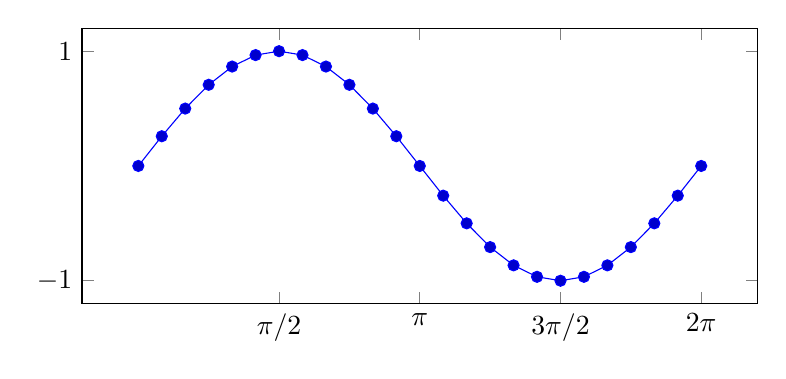
\begin{tikzpicture}
          \begin{axis}[xtick={pi/2,pi,3*pi/2,2*pi},
            xticklabels={$\pi/2$,$\pi$, $3\pi/2$,$2 \pi$,},
            ytick={-1, 1}, width=4in, height=2in]
            \addplot+[domain=0:2*pi]{sin(deg(x))};
          \end{axis}
        \end{tikzpicture}
      \end{center}
    \end{solution}

  \item
    \begin{problem}[\stretch{1}]
      At how many values of $x$ in $[0, 2\pi]$ is $\sin x = 0.7$?
    \end{problem}

    \begin{solution}
      \fbox{2}, since there are two intersections between the graphs of
      $y=\sin(x)$ and $y=0.7$: 
      \begin{center}
        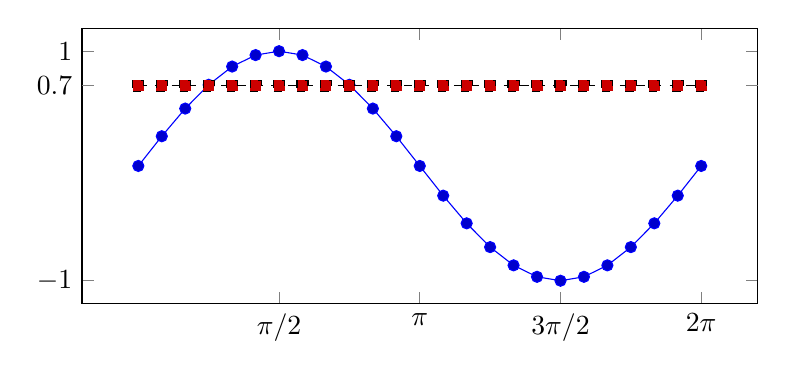
\begin{tikzpicture}
          \begin{axis}[xtick={pi/2,pi,3*pi/2,2*pi},
            xticklabels={$\pi/2$,$\pi$, $3\pi/2$,$2 \pi$,},
            ytick={-1, 1}, width=4in, height=2in, extra y ticks = {0.7}]
            \addplot+[domain=0:2*pi]{sin(deg(x))};
            \addplot+[dashed,black,domain=0:2*pi]{0.7};
          \end{axis}
        \end{tikzpicture}
      \end{center}
    \end{solution}

  \item
\begin{problem}[\stretch{2}]
      Find all values of $x$ in $[0, 2\pi]$ for which $\sin x = 0.7$;
      give exact values as well as numerical approximations, and label
      these values on your graph (on the $x$-axis). One of these is
      $\arcsin 0.7$. The other you need to write in terms of $\arcsin 0.7$.
      The unit circle is your friend!
    \end{problem}

    \begin{solution}
      We know one solution of $\sin x = 0.7$, $x = \arcsin(0.7)$.  Let's
      call this $A$. Remember that $A = \arcsin(0.7)$ is the angle in
      $\left[ - \frac{\pi}{2}, \frac{\pi}{2} \right]$ whose sine is $0.7$;
      we can picture it like this:
      \begin{center}
        \begin{tikzangle}[angle=rad(asin(0.7)), label=$A$, color=blue,
          func=sin, functick={$0.7$}]
          \draw[blue] (axis cs: 1.5, 0) node[right] {$A = \arcsin 0.7$}; 
        \end{tikzangle}
      \end{center}
      (In particular, since $A$ must be in $\left[ - \frac{\pi}{2},
        \frac{\pi}{2} \right]$ and $\sin A$ is positive, $A$ is between
      $0$ and $\frac{\pi}{2}$.)  Now, we can picture all values of $x$ in
      $[0, 2 \pi]$ such that $\sin x = 0.7$ and express these in terms
      of $A$.  The possible angles $x$ are shown below:
      \begin{center}
      \begin{tikzpicture}
        \begin{axis}[axis equal=true, 
          xmin=-1.3, xmax=1.3, ymin=-1.3, ymax=1.3, clip=false,
          xtick=\empty, ytick=\empty, extra y ticks={0.7}, width=3in,
          set layers=tick labels on top]
          \coordinate (O) at (0,0);
          \coordinate (A) at (1,0);
          \coordinate (R) at (\rtheta{1}{44.43});
          \coordinate (P) at (\rtheta{1}{135.57});
          \addplot[domain=0:360, data cs=polar] (x,1);
          \draw[thick,blue] (O) -- (R);
          \draw[thick,red] (O) -- (P);
          \filldraw[fill=blue,radius=2pt] (R) circle;
          \filldraw[fill=red,radius=2pt] (P) circle;
          \draw pic[text=blue,draw=blue,thick,angle radius=18,
          "\normalsize$A$",angle eccentricity=1.4]
          {angle=A--O--R};
          \draw pic[text=red,draw=red,thick,angle radius=10,
          "\normalsize$\pi-A$",angle eccentricity = 1.8]
          {angle=A--O--P};
        \end{axis}
      \end{tikzpicture}
      \end{center}
     So, the two solutions are $\boxed{\arcsin (0.7) \text{ and }
        \pi - \arcsin (0.7)}$.  Using a calculator, these are 
      $\boxed{\approx 0.78, 2.37}$.  Here they are labeled on
      the graph of $\sin x$ we drew earlier: 
      \begin{center}
        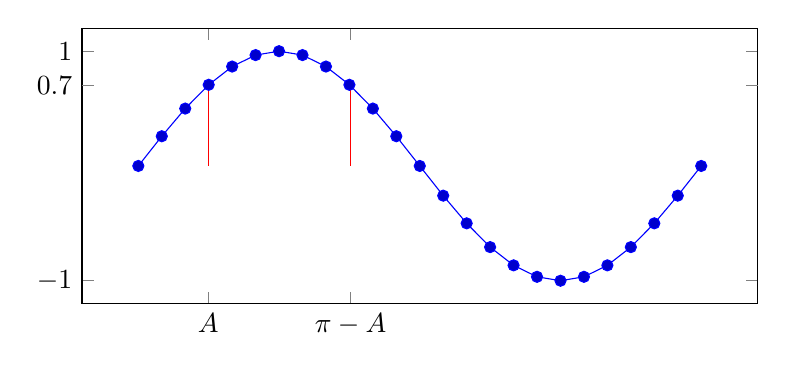
\begin{tikzpicture}
          \begin{axis}[xtick={0.78, 2.37}, xticklabels={$A$,
              $\pi - A$}, ytick={-1, 1},
            width=4in, height=2in, extra y ticks={0.7}] %
            \addplot+[domain=0:2*pi]{sin(deg(x))};
            \pgfplotsforeachungrouped \x in {0.78, 2.37}
            {
              \edef\temp{%
                \noexpand\draw[red] (axis cs: \x, 0) -- (axis cs: \x, 0.7); %
              }
              \temp
            }
          \end{axis}
        \end{tikzpicture}
      \end{center}
    \end{solution}

  \item
    \begin{problem}[\nstretch{2}]
      Find all values of $x$ in $[0, 4\pi]$ for which $\sin x = -0.7$;
      give exact values as well as numerical approximations. Graph
      $y=\sin x$ on $[0,4\pi]$ and make sure you got all values.
    \end{problem}

    \begin{solution}
    \begin{center}
        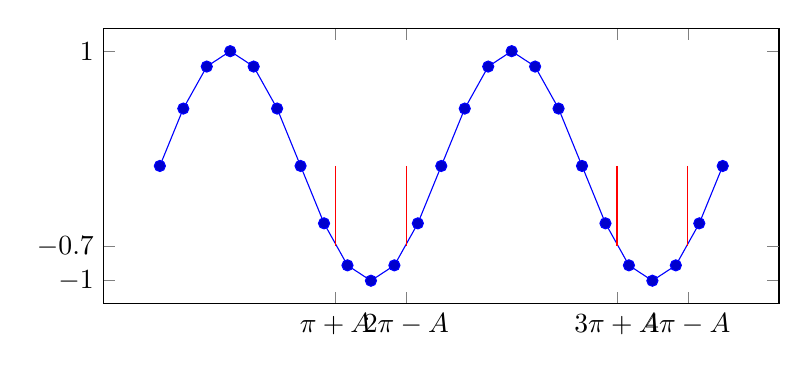
\begin{tikzpicture}
          \begin{axis}[xtick={pi+0.78,2*pi-0.78,3*pi+0.78,4*pi-0.78},
          xticklabels={$\pi+A$, $2\pi - A$, $3\pi+A$, $4\pi-A$}, ytick={-1, 1},
            width=4in, height=2in, extra y ticks={-0.7}] %
            \addplot+[domain=0:4*pi]{sin(deg(x))};
            \pgfplotsforeachungrouped \x in {pi+0.78,2*pi-0.78,3*pi+0.78, 4*pi-0.78}
            {
              \edef\temp{%
                \noexpand\draw[red] (axis cs: \x, 0) -- (axis cs: \x, -0.7); %
              }
              \temp
            }
          \end{axis}
        \end{tikzpicture}
      \end{center}
      Based on the graph, there are 4 such values of $x$.  Let's express them in terms of $A =
      \arcsin(0.7)$:
      \begin{center}
        \begin{tabular}{cccc}
          \begin{tikzangle}[angle=pi+rad(asin(0.7)), label=$x$,
            func=sin, ytick={-0.7, 0.7}, yticklabels={},
            secondangle=rad(asin(0.7)), secondlabel=$A$, seconddistance=0.25] % 
            \draw[funcline] (axis cs: 0.714, 0.7) -- (axis cs: -0.714, 0.7); %
            \draw (axis cs: 0, -0.7) node[funcxtick]{$-0.7$}; %             
            \draw (axis cs: 0, 0.7) node[funcxtick]{$0.7$}; %
          \end{tikzangle} & 
          \begin{tikzangle}[angle=2*pi-rad(asin(0.7)), label=$x$,
            func=sin, ytick={-0.7, 0.7},
            secondangle=rad(asin(0.7)), secondlabel=$A$, seconddistance=0.25] % 
            \draw[funcline] (axis cs: 0.714, 0.7) -- (axis cs: -0.714, 0.7); %
            \draw (axis cs: 0, -0.7) node[funcxtick]{$-0.7$}; %             
            \draw (axis cs: 0, 0.7) node[funcxtick]{$0.7$}; %
          \end{tikzangle} & 
          \begin{tikzangle}[angle=3*pi+rad(asin(0.7)), label=$x$,
            func=sin, ytick={-0.7, 0.7},
            secondangle=rad(asin(0.7)), secondlabel=$A$, seconddistance=0.25] % 
            \draw[funcline] (axis cs: 0.714, 0.7) -- (axis cs: -0.714, 0.7); %
            \draw (axis cs: 0, -0.7) node[funcxtick]{$-0.7$}; %             
            \draw (axis cs: 0, 0.7) node[funcxtick]{$0.7$}; %
          \end{tikzangle} & 
          \begin{tikzangle}[angle=4*pi-rad(asin(0.7)), label=$x$,
            func=sin, ytick={-0.7, 0.7},
            secondangle=rad(asin(0.7)), secondlabel=$A$, seconddistance=0.25] % 
            \draw[funcline] (axis cs: 0.714, 0.7) -- (axis cs: -0.714, 0.7); %
            \draw (axis cs: 0, -0.7) node[funcxtick]{$-0.7$}; %             
            \draw (axis cs: 0, 0.7) node[funcxtick]{$0.7$}; %
          \end{tikzangle} \\
          $x = \pi + A$ & $x = 2\pi-A$ & $x = 3\pi+A$ & $x = 4\pi - A$
        \end{tabular}
      \end{center}
      So, the four solutions are $\boxed{\pi + \arcsin (0.7), 2\pi -
        \arcsin(0.7), 3\pi + \arcsin(0.7), 4 \pi - \arcsin(0.7)}$.  These
      are $\boxed{\approx 3.92, 5.51, 10.2, 11.8}$.         
    \end{solution}

  \end{enumerate}



\item 

\begin{grading}
 5 points:   3 for part (a) and 2 for part (b).
\end{grading}

 \textbf{Reflect Back.}

  \begin{enumerate}[topsep=0pt]
  \item
    \begin{problem}[\vfill]
      Silvio knows from using a calculator that $\sin 2.5
      \approx 0.6$.  He says,
      \begin{quote}
        ``Since $\sin 2.5 \approx 0.6$, if I take the $\arcsin$ of
        both sides, I get that $\arcsin 0.6 \approx 2.5$.''
      \end{quote}
      What's wrong with Silvio's reasoning?
    \end{problem}

    \begin{solution}
      First, Silvio's answer is wrong because $\arcsin 0.6$ is defined to
      be the angle \hl{\textbf{in $\bm{\left[ - \frac{\pi}{2},
              \frac{\pi}{2} \right]}$}} whose sine is $0.6$, and $2.5$ is
      not in $\left[ - \frac{\pi}{2}, \frac{\pi}{2}
      \right]$.  

      The problem with Silvio's reasoning is that, when he takes the
      $\arcsin$ of both sides, he gets
      \[ \arcsin(\sin 2.5) \approx \arcsin \left( 0.6 \right).\] However,
      it's not true that $\arcsin(\sin(2.5)) = 2.5$; as we saw in
      {{\#7}} on the worksheet, $\arcsin(\sin x)$ is only equal to $x$ for
      $x$ in $\left[ - \frac{\pi}{2}, \frac{\pi}{2} \right]$.
    \end{solution}

  \item
    \begin{problem}[\vfill]
      $\arcsin x$ is defined to be the angle in $\left[ - \frac{\pi}{2},
        \frac{\pi}{2} \right]$ whose sine value is $x$.  Why do we not
      similarly define $\arccos x$ to be the angle in $\left[ -
        \frac{\pi}{2}, \frac{\pi}{2} \right]$ whose cosine value is $x$?
    \end{problem}

    \begin{solution}
      This would not be a function; for example, there are two angles in
      $\left[ - \frac{\pi}{2}, \frac{\pi}{2} \right]$ whose cosine value
      is $\frac{1}{2}$: $\pm \frac{\pi}{3}$.  Additionally, the arccosine of negative values would not be defined.
    \end{solution}

  \end{enumerate}

% \item 

% \begin{grading}
%  5 points extra credit. 
% \end{grading}

%  (Optional extra credit, 5 points)
% As you saw in {{{Problem Set 9}, {{\#7}}}}, the Greek mathematician
%   Eratosthenes was able to estimate the circumference of the earth in 200
%   BC by comparing shadows at Alexandria and Syene.  Here's what
%   Eratosthenes knew:
%   \begin{itemize}[topsep=0pt]
%   \item At noon on June 21, the sun was directly overhead at Syene, so
%     that a vertical stick in the ground cast no shadow.
%   \item At the same moment in Alexandria, a 1-meter tall stick cast a
%     shadow of length 0.126 meters on the ground.
%   \item The distance for a man to walk directly from Alexandria to Syene
%     was 800 km.\footnote{Legends vary on how Eratosthenes determined this
%       distance; some say he hired someone to count the paces between the
%       cities; others say he found it by multiplying the time it took for a
%       camel caravan to travel between the cities by the speed of the
%       caravan.}
%   \end{itemize}
%   Finally, Eratosthenes assumed that the sun was so far away from the
%   Earth that its rays at Alexandria and Syene could be considered parallel.

%     \pspace{\newpage}

%    The diagram below shows the sun
%   shining on the Earth at noon on June 21, with sticks at Alexandria
%   (point A) and Syene (point S).

%   \begin{center}
%     \begin{tikzpicture}[scale=0.7]
%       \pgfmathsetmacro{\A}{90};
%       \pgfmathsetmacro{\S}{60};
%       \draw (0, 0) circle(3);
%       \begin{scope}[blue, very thick]
%         \draw (\A: 3) -- (\A: 3.5);
%         \draw (\S: 3) -- (\S: 3.5);        
%       \end{scope}
%       \begin{scope}[orange]
%         \foreach \x in {0, 0.51, ..., 2.04}
%         {
%           \draw ($(\S: 5) - (\x, 0)$) -- ++ ({-1.5*cos(\S)}, {-1.5*sin(\S)});
%         }
%         \path (\S: 5) -- node[right]{sun's rays} ++ ({-1.5*cos(\S)}, {-1.5*sin(\S)});        
%       \end{scope}
%       \draw[gray, dashed] (\A: 3) -- (0, 0) -- (\S: 3);
%       \filldraw (\A: 3) circle(2pt) node[anchor=north east]{A};
%       \filldraw (\S: 3) circle(2pt) node[below]{S};
%     \end{tikzpicture}
%   \end{center}

%   How can you put this information together to find the circumference of
%   the Earth?

%   \pspace{\vfill}

%   \begin{solution}
%     The key, as Eratosthenes realized, was to look at the shadow of the
%     stick at Alexandria; that's the red length in the diagram below.
%     Notice that there's now a small right triangle whose legs are the
%     stick and the shadow.  Let's also label the angle between the two gray
%     lines $\theta$:

%     \begin{center}
%       \begin{tikzpicture}
%         \pgfmathsetmacro{\A}{90};
%         \pgfmathsetmacro{\S}{60};
%         \draw (0, 0) circle(3);
%         \begin{scope}[blue, very thick]
%           \draw (\A: 3) -- (\A: 3.5);
%           \draw (\S: 3) -- (\S: 3.5);        
%         \end{scope}
%         \draw[red, very thick] (\A: 3) -- +({-0.5/sqrt(3)}, 0);
%         \begin{scope}[orange]
%           \foreach \x in {0, 0.51, ..., 2.04}
%           {
%             \draw ($(\S: 5) - (\x, 0)$) -- ++ ({-1.5*cos(\S)}, {-1.5*sin(\S)});
%           }
%           \path (\S: 5) -- node[right]{sun's rays} ++ ({-1.5*cos(\S)}, {-1.5*sin(\S)});        
%         \end{scope}
%         \draw[gray, dashed] (\A: 3) -- (0, 0) -- (\S: 3);
%         \filldraw (\A: 3) circle(2pt) node[anchor=north east]{A};
%         \filldraw (\S: 3) circle(2pt) node[below]{S};
%         \draw (0, 8pt) arc[radius=8pt, start angle=\A, end angle=\S];
%         \draw (75: 16pt) node{$\theta$};
%       \end{tikzpicture}
%     \end{center}
%     Because the sun's rays are parallel to the gray line from Syene to the
%     center of the earth, the top angle in the right triangle is also
%     $\theta$; here's an enlarged version of the triangle:
%     \begin{center}
%       \begin{tikzpicture}[x=6cm, y=6cm]
%         \pgfmathsetmacro{\A}{90};
%         \pgfmathsetmacro{\S}{60};
%         \draw[blue, very thick] (\A: 3) -- node[right] {1 m stick} (\A: 3.5);
%         \draw[red, very thick] (\A: 3) -- node[below] {0.126 m shadow} +({-0.5/sqrt(3)}, 0);
%         \draw[orange] ($(\A: 3) + ({-0.5/sqrt(3)}, 0)$) -- (\A: 3.5);
%         \draw ($(\A: 3.5) - (0, 8pt)$) arc[radius=8pt, start angle=270,
%         end angle=240];
%         \draw ($(\A: 3.5) + (255: 16pt)$) node{$\theta$};
%       \end{tikzpicture}
%     \end{center}
%     From the right triangle, $\tan \theta = \frac{0.126}{1} = 0.126$.
%     Since $\theta$ is an acute angle, 
%     $\theta \approx \arctan (0.126) \approx 0.125$ radians.

%     Now, let's go back to the picture of the earth; the arc between
%     Alexandria and Syene subtends an angle of $\theta \approx 0.125$
%     radians, so it is a fraction $\frac{0.125}{2 \pi}$ of the whole
%     circle.  On the other hand, its length is 800 km, so we've figured out
%     \begin{align*}
%       800 &\approx \frac{0.125}{2 \pi} \text{(circumference of Earth)},
%     \end{align*}
%     which means the circumference of the Earth is about $\frac{800 \cdot
%       2\pi}{0.125} = \frac{1600 \pi}{0.125} \approx \boxed{40103\text{
%         km}}$.  (This is extremely close to the modern accepted
%     measurement of 40,075 km for the circumference of the earth around the
%     equator!)
%   \end{solution}  

\end{enumerate}

\psreflection{

  Optional reading for next class is \S20.4 in Gottlieb.}
\end{document}